\documentclass[12pt]{article}
	\usepackage{mgates-letter}
	\definecolor{dark_blue} {rgb}{0., 0., 0.65}
	
	\usepackage{textcomp}
	\usepackage{mathrsfs}  % mathscr font
	\usepackage{boxedminipage}
	\usepackage{rotating}
	\usepackage{svg}
	%\usepackage{natbib}
	\usepackage[colorlinks, filecolor=dark_blue, urlcolor=dark_blue, linkcolor=black, citecolor=black]{hyperref}
\begin{document}

\title{Towards democratization and resource awareness in dynamic swarm behaviors}
\author{Leonardo Micelli}
\date{\today}
\maketitle

\noindent


% ----------------------------------------
\newpage
\setcounter{tocdepth}{2}

% set these after the TOC
\setlength{\parindent}{0em}
\setlength{\parskip}{1em}

% ----------------------------------------
\section{State of the Art}
\paragraph{\textbf{Collective Adaptive Systems and Macroprogramming}} Collective Adaptive Systems~\cite{ferscha2015collective} are large scale distributed systems composed of multiple autonomous, 
interacting entities that operate in open-ended environments. While each entity within the CAS (i.e. sensor, robot, software agent) operates autonomously with its own local context and objective, their interactions
produce \textbf{emergent global behaviors}. Decision-making in CAS is decentralized, and global functionality emerges from local interaction. Examples of CAS can be found in \textit{Smart Cities}, \textit{WSNs}, \textit{Digital Twins} and \textit{Swarm Robotics}.
CAS are tipically heterogeneous and highly dynamic: entities can fail, join and leave at any time, introducing key challenges ranging from scalability and resource constraints to resilience and adaptability in
unpredictable environments. Novel approaches to the engineering of CAS propose to shift the focus from the individual entity to the collective as a whole \textit{(macroprogramming~\cite{10.1145/3579353})}, to manage increasing complexity while
improving maintainability. The main idea is to capture the macroscopic behavior of a collective system through a single program, abstracting away the complexities of individual components.

\paragraph{\textbf{Swarm Robotics}} Swarm robotics is an approach to collective robotics that draws inspiration from the self-organized behavior of social animals ~\cite{brambilla2013swarm}. The goal is to design robust, flexible and scalable 
collective behaviors for large number of robots through simple rules and local interactions. There are two main methods for designing such systems: \textit{automatic design}, which employs methods derived from
evolutionary robotics and multi-robot reinforcement learning, and \textit{behavior-based design}, which involves the design and implementation of algorithms that can be executed by the robots. This design approach is often realized
in a bottom-up fashion, starting from the individual behavior of the robots. Conversely, the top-down approach is based on the idea of expressing the desired behavior of the swarm by expressing a set of instruction at the collective level.
Another important distinction is between \textit{centralized} and \textit{decentralized} approaches. Centralized approaches rely on a central entity that coordinates the behavior of the swarm, while decentralized approaches rely on local interactions between the robots to achieve the desired behavior.
Decentralized approaches, in particular, offer several interesting properties such as robustness, fault tolerance and scalability, while centralized approaches are often more efficient and easier to implement.
The field of swarm robotics has found several applications in various domains, such as \textit{(i)} foraging, \textit{(ii)} surveillance, \textit{(iii)} exploration, \textit{(iv)} transportation and logistics.


\paragraph{\textbf{Aggregate Computing and Field Calculus}} AC~\cite{beal2016aggregate} is a macroprogramming approach that aims to ease the engineering of CAS by shifting the
focus from the individual device perspective to large aggregations of devices. It does so by exploiting the concepts of computational fields and FC.
Within the FC, a computational field is a function mapping every computational device in a network, represented by a dynamic and reflexive neighboring
relationship between devices, to a computational object. The main goal is to express the aggregate system behavior
through a functional composition of fundamental operators that manipulate (evolve, combine, restrict)
computational fields. A key concept of Field Calculus is that these aggregate-level specifications can
also be interpreted as a local set of rules that define the iterative asynchronous execution of computation rounds.

TODO: si potrebbe riformulare spiegando più nel dettaglio event structures e i self-stabilizing operators???

\paragraph{\textbf{Aggregate Computing Incarnations}} Research on AC has led to the development of several incarnations, each of them tackling various research challenges of AC.
\textit{Scafi}~\cite{casadei2016towards} is one of the most actively researched and maintained implementations of
AC. It is hosted in the Scala language, a powerful and expressive JVM-based language. The main advantage of Scafi is its ability to provide a
more high-level platform to support agile prototyping for research. \textit{Collektive} is a Kotlin-based implementation of AC that provides an extension of FC via the eXchange Calculus (XC) ~\cite{audrito2024exchange}.
It provides an expressive DSL and it is natively multi-platform, enabling AC on a wider range of targets.
\textit{FCCP}~\cite{audrito2024fcpp} is a C++ library that implements FC. It has been designed and developed to bring the AC paradigm to
resource-constrained devices that cannot support the JVM. It does so by providing an extensible C++ library and a performance-oriented simulator that allows
the developer to speed up the development process of aggregate programs.

%\paragraph{\textbf{MacroSwarm}} The analysis from Brambilla~\cite{brambilla2013swarm} highlighted a gap in research on top-down design methods of collective behaviors and a problem of
%formal verification and validation, heterogeneity and operational/maintenance issues.  
%MacroSwarm~\cite{aguzzi2023macroswarm} is a computational field-based coordination approach with the goal of enabling the design and development of swarm robotic systems by
%providing reusable and fully composable functional components embedding collective computation and coordination, based on the macroprogramming paradigm of AC.
%The main idea of MacroSwarm is to express each swarm behavior block as a pure function mapping sensing fields to actuation fields, including movement vectors.
%The main API of MacroSwarm consists of an extension of the Scafi DSL that provides functional blocks covering key swarming patterns, such as \textit{(i)} flocking, \textit{(ii)} pattern formation, \textit{(iii)} consensus and \textit{(iv)} leader-follower behaviors, 
%all of which backed by the formal framework of AC, for which self-stabilisation properties are guaranteed. This allows MacroSwarm operators to enjoy formally captured resiliency properties.
%It does so by leveraging self-stabilizing FC operators such as \textit{(i) Sparse choice} (leader election), \textit{(ii) Gradient-cast} (distributed propagation) and \textit{(iii) Collect-cast} (distributed collection).
 

\subsection{Coherence with my previous academic experience}
\label{sec:coherence}
This proposed research projects extends and builds upon my previous academic experience, in particular in my last year of Master's degree.
I have been introduced to AC and Scafi during the course of "Pervasive computing". Here, in the context of the final examination project for the course,
I worked alongside three colleagues of mine to develop a Rust-based imlpementation of Aggregate Computing and a Scala 3 port of the Scafi DSL.
I then built upon this project to develop my Master's thesis where I proposed a Rust-based distributed framework to execute distributed AC programs in a network of
heterogeneous devices, with the main goal of democratizing AC by offering a high-level API that can be supported in resource-constrained devices.

% ----------------------------------------
\section{Description of the Project}
\subsection{Motivation}
%The coordination of distributed agents in dynamic and uncertain environments is a longstanding challenge in the design of collective adaptive systems. 
%Recent advances in Aggregate Computing (AC) have provided powerful abstractions for expressing global behaviour through local interactions.
%In particular, state-of-the-art swarm robotics approaches, such as MacroSwarm can leverage self-stabilisation properties of AC operators to enable
%the design of robust and resilient collective behaviors, showing promise on a AC-based approach to swarm robotics.
%However, important gaps remain in terms of dynamic team formation, dynamic collective resource management and adaptive workflow management and planning.
%Furthermore, reliance on predominantly JVM-based architectures shows limitations in terms of democratization of the proposed approaches, as they are not easily deployable on resource-constrained devices.
The analysis from Brambilla~\cite{brambilla2013swarm} highlighted a gap in research on top-down design methods of collective behaviors and a problem of
formal verification and validation, heterogeneity and operational/maintenance issues. There is still a lack of formal, general and ergonomic approaches to swarm behaviors,
and solutions that take can be deployed in real-world, resource-constrained contexts are yet to be researched. There has been a recent rise in research contribution on the matter, 
particularly with the Scafi-based framework Macroswarm~\cite{aguzzi2023macroswarm}, which takes advantage of self-stabilising FC constructs and the expressiveness provided from the
Scafi DSL to offer an API consisting of functional, composable building blocks of swarm behavior.
However, important gaps remain in terms of dynamic team formation, dynamic collective resource management and adaptive workflow management and planning.
Furthermore, reliance on predominantly JVM-based architectures shows limitations in terms of democratization of the proposed approaches, as they are not easily deployable on resource-constrained devices tipically
found in real-world scenarios, confining recent developments to simulations.

\subsection{Idea}
%The idea of the project, exemplified in Figure~\ref{fig:research-project}, is to build upon and extend the theoretical and practical foundations of Aggregate Computing to address scenarios where team composition, 
%task allocation, and resource availability evolve at runtime. In such contexts, ranging from swarms of heterogeneous robots to decentralized sensor-actuator 
%systems, collectives must continuously reconfigure in response to failures, environmental changes, or shifting goals.

%In particular, the research idea is to explore new computational constructs and coordination mechanisms that:
%\textit{(i)} enable dynamic team formation among distributed agents based on context and capability, 
%\textit{(ii)} support resilient task execution and workflow adaptation under partial knowledge and failures and
%\textit{(iii)} integrate resource-awareness and management into aggregate programs, allowing systems to self-optimize across heterogeneous hardware and network conditions.

%These directions aim to bridge the gap between the high-level expressiveness of aggregate programming and the operational realities of constrained, distributed environments. 
%By enriching the AC paradigm with notions of runtime adaptation, team-level abstractions, and workflow semantics, this work intends to push the boundaries of what is currently 
%achievable in terms of autonomy and coordination in collective systems.

%To support this vision, a secondary—but relevant—objective is to further investigate a lightweight and accessible AC platform that enables the deployment of these advanced coordination strategies 
%on resource-constrained devices. A native implementation, potentially based on Rust, could make aggregate models usable in domains currently underserved by JVM-based solutions, 
%facilitating real-world validation and promoting wider adoption.

%Ultimately, this project aims to make a conceptual and methodological contribution to the field of collective adaptive systems, by redefining how dynamic workflows, resilience, and resource-awareness 
%can be expressed and executed within the aggregate computing paradigm in the swarm robotics context.


The idea of the project, exemplified in Figure~\ref{fig:research-project}, is to provide a top-down, behavior-based and FC-powered approach to swarm robotics engineering, by offering a
resilient, functional and composable general purpose API.
At the base of the project lies a "democratic" Aggregate Computing incarnation. Here the goal is to provide a high-level DSL as in the most recent discussed AC incarnations,
while preserving the ability to be deployed in resource-constrained environments. The platform will expose well-researched, self-stabilizing FC constructs such as
\textit{(i) Sparse choice S} (leader election), \textit{(ii) Gradient-cast G} (distributed propagation) and \textit{(iii) Collect-cast C} (distributed collection) that will be used to form
the base blocks for swarm behavior. The solution will also build upon and extend the theoretical and practical foundations of Aggregate Computing to address scenarios where team composition, 
task allocation, and resource availability evolve at runtime. In such contexts, ranging from swarms of heterogeneous robots to decentralized sensor-actuator 
systems, collectives must continuously reconfigure in response to failures, environmental changes, or shifting goals.

\begin{figure}
	\centering
	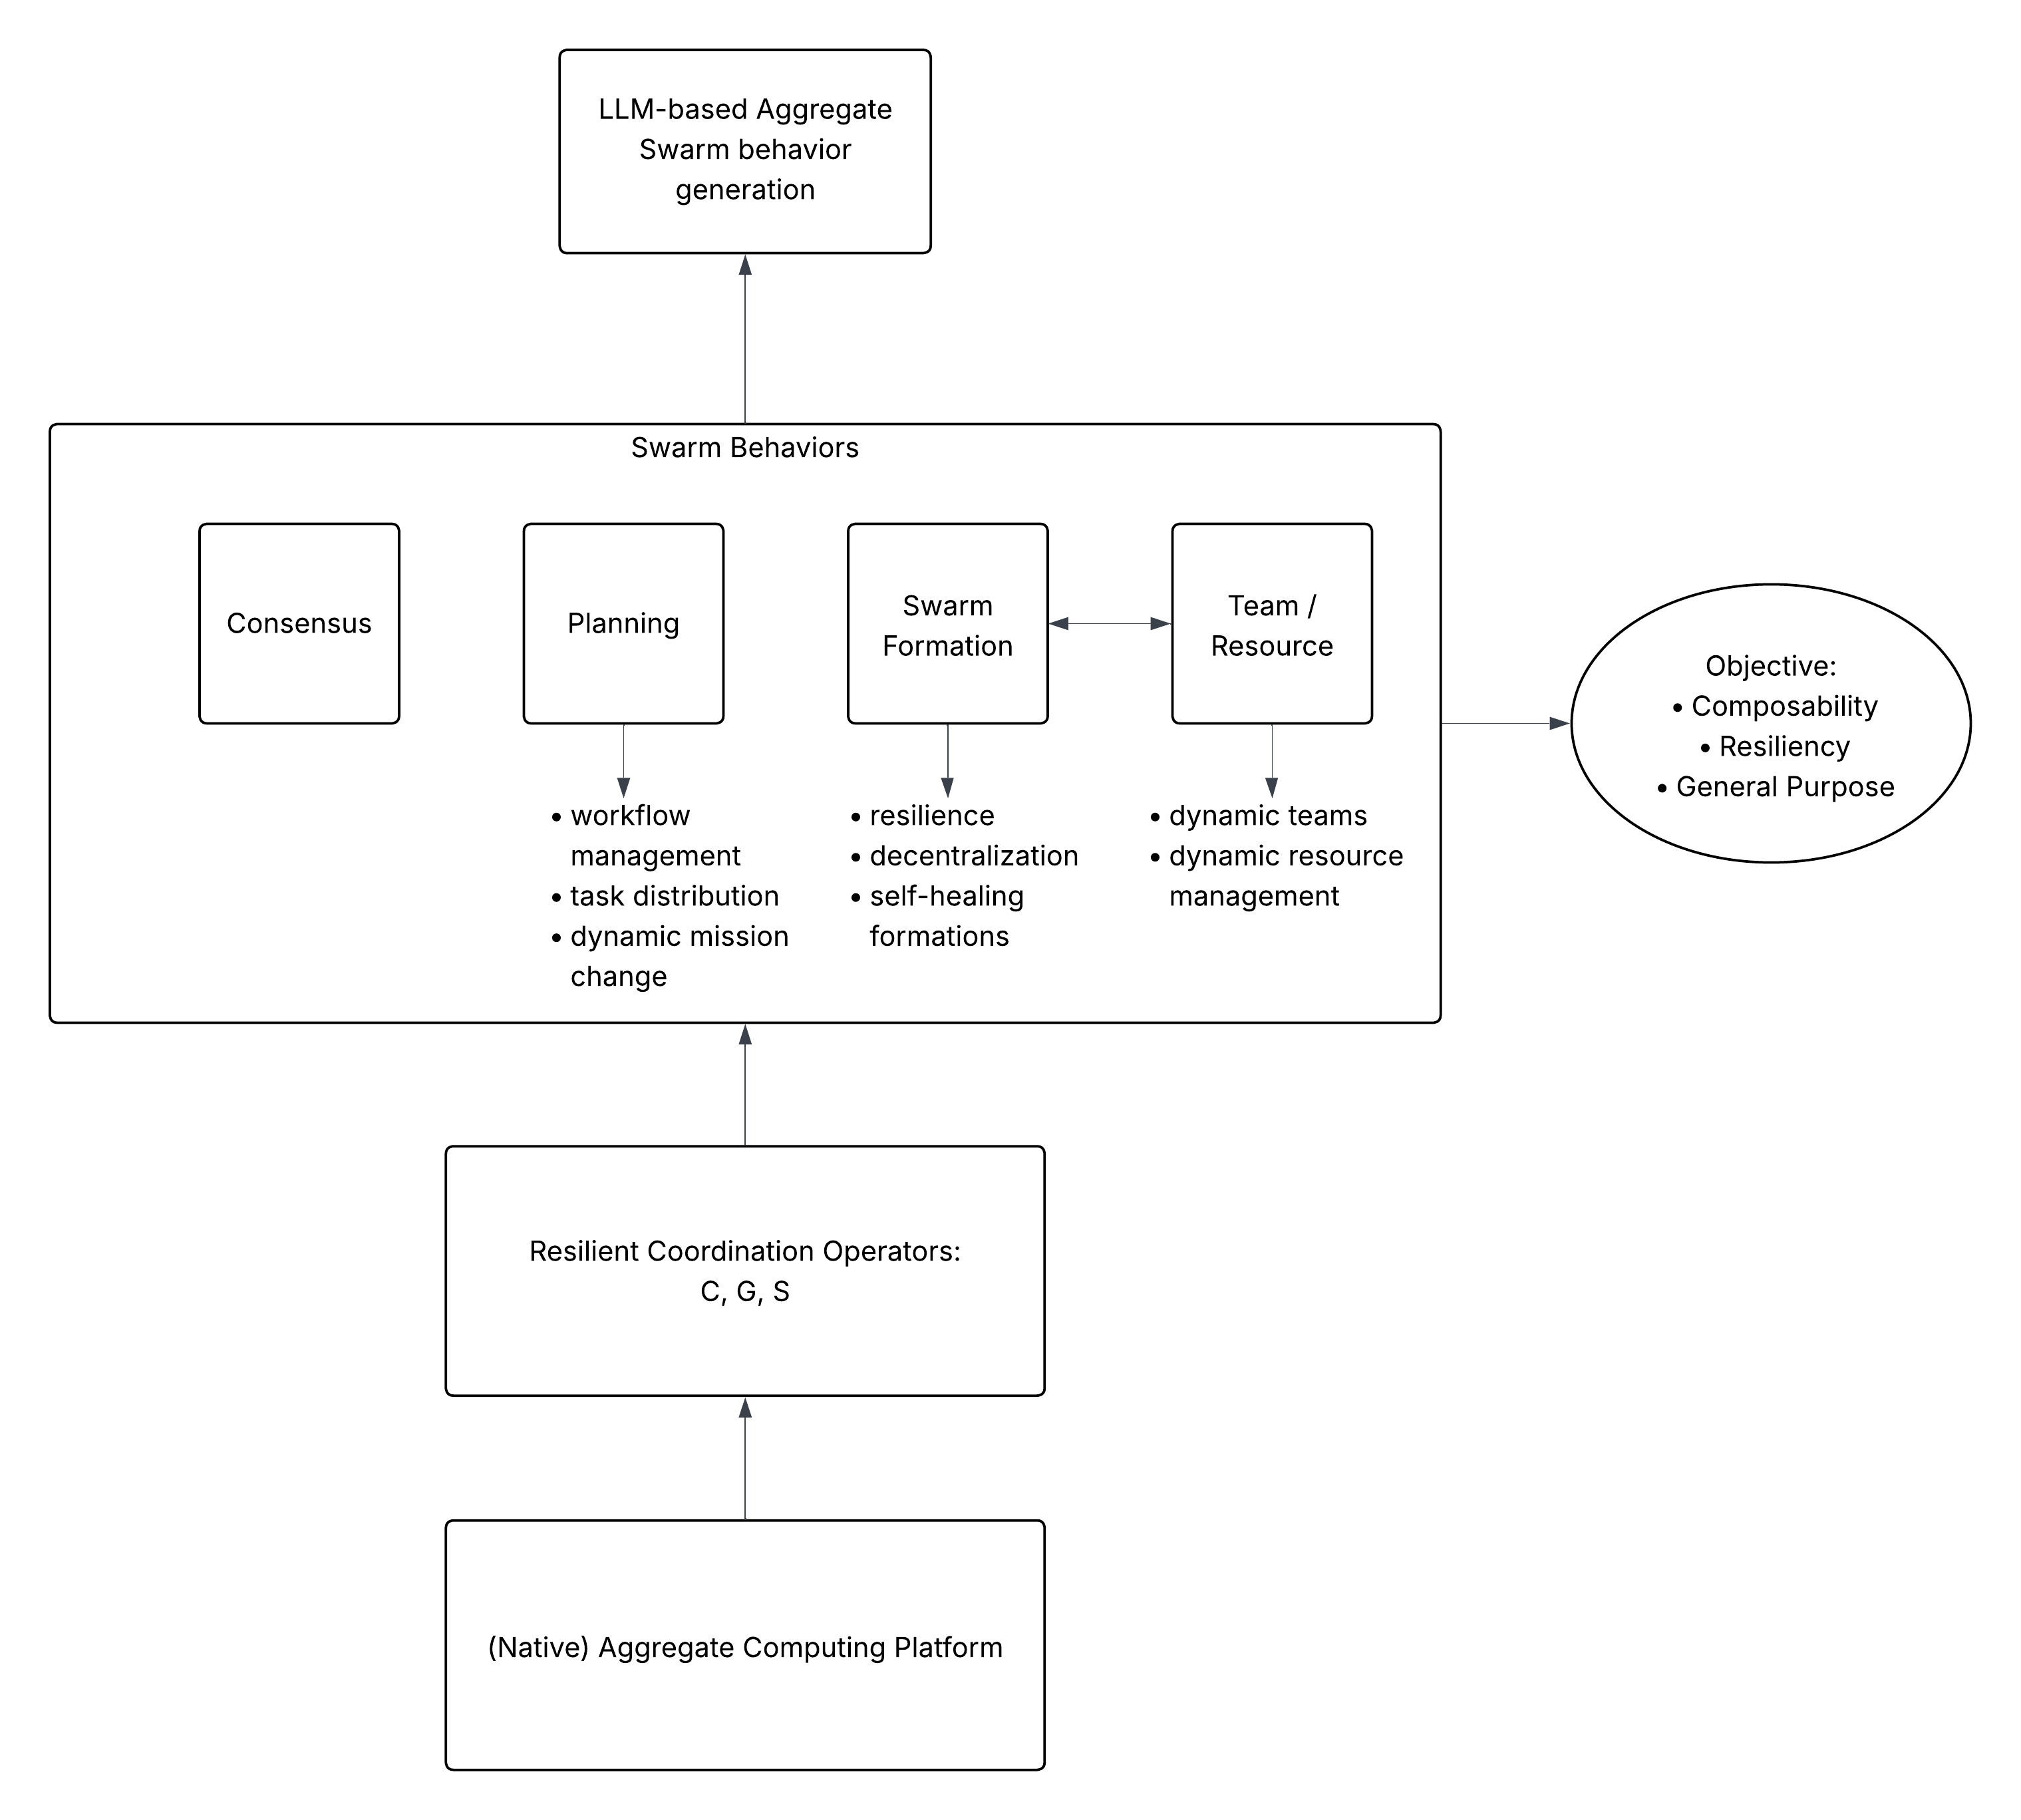
\includegraphics[width=0.7\textwidth]{figures/ResearchProject.png}
	\caption{Overview of the research project}
	 \label{fig:research-project}
\end{figure}

\subsection{Research Goals and Challenges}
\label{sec:challenges}

\subsubsection{Team Management}
CAS are naturally dynamic and continually evolving. One implication of these properties is that entities within a CAS can fail, join and leave over the course of time.
Within a collective computation and AC, the sudden change in the neighborhood of the composing entities can yield to different outputs, and this effect may propagate upwards and
affect the collective result of the computation. In AC-based swarm robotic contexts, where swarm behaviors are mappings between sensing fields to actuation fields, sudden changes
in the actual underlying network of robots can cause the inability of the entire system to reach the desired collective goal. Ensuring that the swarm behavior expressed through the
framework is resilient to sudden topology change is crucial to provide stable behavior. 

\subsubsection{Resource Management}
Most robots in swarms are resource-constrained (small drones with limited battery, etc.). An open challenge is how to extend swarm operation time and range. 
Some recent research focuses on energy-aware swarm algorithms e.g., task allocation that accounts for remaining battery, or formation flying that lets some drones draft off others to save power (much like geese in a V formation). 
Swarms might employ rotation strategies, where robots take turns performing power-intensive tasks versus idle roles, to maximize overall mission duration.
Possible decentralized approaches to the problem may be market-based solutions, where tasks may be auctioned and costed based on local condition.

\subsubsection{Swarm Formation}
Team formation patterns are one of the key challenges of engineering swarm behaviors. 
Teams can be formed from the swarm following a particular logic, sensor reading or spatial structure. Usually teams 
are associated to a leader (introducing the challenge of \textit{leader election}) which can function as an area of influence in the
local decision of the neighboring nodes. Recent research show the need of advancements in the following categories:
\textit{(i) decentralization}: the formation behavior needs to emerge from local interaction between robots in the swarm, rather than from a centralized entity. 
\textit{(ii) resilience}, meaning the ability of the swarm to maintain formation/decision
in the presence of adversarial events, in particular \textit{message loss, perception position errors} and \textit{node failures}.
\textit{(iii) self-healing}, i.e. the ability of the formation to reconstruct itself and return to a stable structure if disturbances in the structure happen. Recent progress has been made
regarding self-healing structures, in particular MacroSwarm offers a set of structures that have been proven as self-healing. However, deeper research in the topic is needed to generalize self-healing
to all possible swarm formation structures.

\subsubsection{Planning}
Planning in swarm robotics is the distributed process by which the collective dynamically coordinates their actions to achieve complex, adaptive objectives.
In top-down, macro level approaches, it is possible to devise an algorithm expressing the collective goal of the swarm by combining swarm behaviors with goals represented by boolean conditions.
While this approach shows a step in the right direction, swarms may be deployed in highly mutable environments, where plan adaptivity and dynamic resource allocation based on environmental conditions
are crucial to allow the swarm to reach its final goal. Nodes may distribute themselves across different independent tasks based on local status and condition, or may adapt their current global behavior
based on available resources in order to prevent wear-off or save energy.
This highlights the need for a mechanism to express resource, condition aware plans and dynamic workflows.

\subsubsection{Democratization of Aggregate Computing}
%caratteristiche di democratic AC. Rustfields?
In the context of the proposed project, a \textit{democratic} incarnation of Aggregate Computing \textit{(i)} provides an expressive, general purpose and
composable API that enables the design, development and maintenance of complex CAS (user-oriented democratization), \textit{(ii)} enables the deployment
in the largest portions of systems, even highly resource-constrained ones (device-oriented democratization). Current AC incarnations offer different properties
regarding this matter, in particular Scafi is highly expressive but with limited device coverage, while FCPP can be deployed in limited resources environments
at the cost of ergonomics. Alongside this spectrum, there are incarnations that have the capability to cover more devices while maintaining expressiveness, such as the Kotlin-based
Collektive framework and other solutions are being explored with Rust-based incarnations as mentioned in Section~\ref{sec:coherence}. It will be crucial to the project
to ensure that the AC platform exploited by the framework provides the aforementioned properties.

\subsection{Reference Scenarios}
\label{sec:scenarios}

\paragraph{Digital Twins of Swarms}

% ----------------------------------------
\section{Expected Results}
As a form of result of the proposed project, it is expected to bring \textit{(i)} scientific contributions to CAS engineering, in particular in swarm robotics and collective behavior through AC,
\textit{(iii)} to realize an actionable top-down design framework based on AC to address the open challenges in Section~\ref{sec:challenges}, \textit{(iii)} a real-world validation possibly based on the reference scenarios in Section~\ref{sec:scenarios}.

The future vision for the project is to enable the building of complex, resilient and dynamic swarm behaviors and deploy them in real-world scenarios, some of which could be \textit{(i)} precision agriculture,
\textit{(ii)} environmental monitoring, \textit{(iii)} logistics and warehousing, \textit{(iv)} disaster response and search, 
\textit{(v)} ubiquitous computing with Swarm Digital Twins.

% ----------------------------------------
\section{Lead-time for implementation}
\begin{figure}
	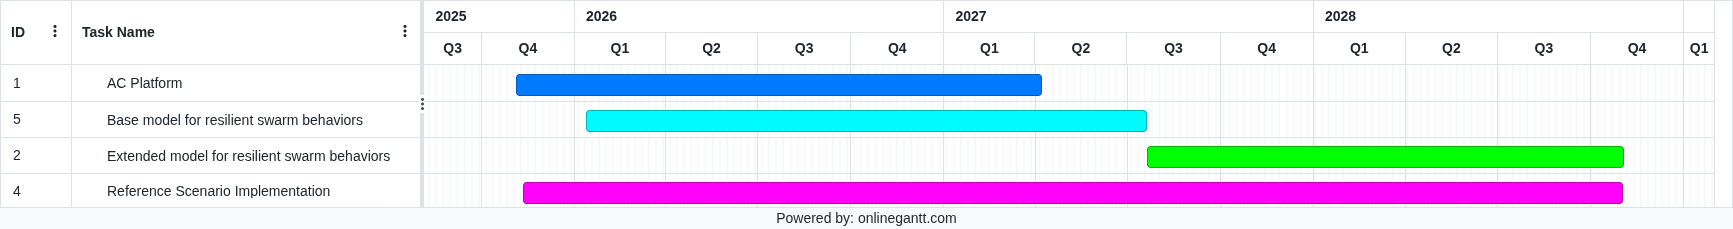
\includegraphics[width=\linewidth]{figures/timeline.png}
	\caption{Hypothetical three year timeline for the project.}
	\label{fig:timeline}
\end{figure}

The Figure~\ref{fig:timeline} shows the hypothetical three-year timeline for the project, subdivided into quarters.

\paragraph{First year.} In the first year will be crucial a deep dive into the research of the state of the art in aggregate computing platforms to devise the design of the Aggregate Computing Platform.
In parallel, deep research of current FC operators and their properties will lay the foundation of the basic composable building blocks for swarm behavior, such as flocking, pattern formation, consensus and leader election.
Due to the overlap of these two tasks, it is expected for the latter to carry over the first half of the second year, to allow enough time for the AC platform to be completed by the end of the first year.

\paragraph{Second year.} Within the second year, it is expected to shift focus from the basic building blocks of swarm behavior to the extended library, that will tackle some of the most relevant challenges expressed in Section~\ref{sec:challenges}.
There will also be an increase in prototyping activities, which will first start in a simulated environment.
Towards the end of the year, it is expected to start leverage swarm behaviors to tackle a reference scenario in the real-world.

\paragraph{Third year.} In the third and final year, the focus will predominantly be to finalize the library of resilient swarm behaviors, while also converging to the end of the real-world testbed in the referenced scenario.

% ----------------------------------------
\section{Proposed criteria to be used to assess the findings obtained}

\paragraph{Qualitative.}
The project will be assessed qualitatively by examining the expressiveness, usability, and resilience of the proposed framework in real-world and simulated deployments.  
Key questions include:  
(i) Expressiveness \& composability: possibility to describe a broad spectrum of swarm behaviours concisely. 
(ii) Robustness \& adaptability in the field: how the swarm copes with adversarial events and whether it self‑stabilises to the intended global behaviour.  
(iii) “Democratisation:” Success is achieved if the same aggregate program can run unmodified on heterogeneous hardware classes that include low resource devices.


\paragraph{Quantitative.}
Experiments need to be rigorously conducted and documented from the beginning of the simulated prototype phase until the end of the reference scenario implementation in the real world.
Detailed quantitative metrics for success need to be expressed while documenting such experiments. 
The metrics gathered will be compared with state-of-the-art swarm robotics frameworks to evaluate performance relative to optimal solutions.
As field-testing requires specialized hardware, efforts will be made to secure partnerships for international research stays during the PhD program, facilitating access to necessary equipment for project testing.

\paragraph{Scientific Contributions.}
During the course of the program, it is expected to contribute to the scientific knowledge of CAS engineering and swarm robotics. 
In particular, it is expected to submit papers annually to conferences that are relevant to the field of CAS (such as ACSOS \footnote{\url{https://acsos.github.io/}}) and robotics (such as ICRA \footnote{\url{https://2025.ieee-icra.org/}}).

\clearpage

%-----------------------------------------
\renewcommand{\refname}{References}

\bibliographystyle{plain}
\bibliography{latex}

\end{document}
